% !TeX spellcheck = pt_BR
\documentclass[tese_patricia]{subfiles}
\begin{document}

% ---------------------------------------------------------- 
% Métodos de malhas sobrepostas
% ----------------------------------------------------------
\chapter[Análise isogeométrica aplicada à Mecânica dos Fluidos]{Análise isogeométrica aplicada à Mecânica dos Fluidos} \label{capitulo:Cap2}
% ----------------------------------------------------------

\nomenclature[C,01]{$p$}{Grau das funções base na direção paramétrica $\xi$;}
\nomenclature[C,02]{$\Xi$}{Vetor de \textit{knots} na direção paramétrica $\xi$;}
\nomenclature[C,03]{$\xi$}{Uma das direções paramémtricas nas quais as funções base são definidas;}
\nomenclature[C,04]{$n$}{Número de funções base na direção paramétrica $\xi$ ;}
\nomenclature[C,05]{$N$}{Função base \textit {B-Spline} na direção paramétrica $\xi$ ;}
\nomenclature[C,06]{$\CP$}{Pontos de controle que descrevem a geometria \textit{B-Spline} ou NURBS;}
\nomenclature[C,07]{$\mathbf{C}$}{Curva \textit {B-Spline} ou NURBS;}
\nomenclature[C,08]{$m$}{Grau das funções base na direção paramétrica $\eta$;}
\nomenclature[C,09]{$\mathcal{H}$}{Vetor de \textit{knots} na direção paramétrica $\eta$;}
\nomenclature[C,10]{$q$}{Número de funções base na direção paramétrica $\eta$ ;}
\nomenclature[C,11]{$\eta$}{Uma das direções paramémtricas nas quais as funções base são definidas;}
\nomenclature[C,12]{$M$}{Função base \textit {B-Spline} na direção paramétrica $\eta$ ;}
\nomenclature[C,13]{$\mathbf{S}$}{Superfície \textit {B-Spline} ou NURBS;}
\nomenclature[C,14]{$\hat{N}$}{Função \textit {B-Spline} fruto do produto tensorial entre funções base descritas em um espaço paramétrico qualquer;}
\nomenclature[C,15]{$L$}{Função base \textit {B-Spline} na direção paramétrica $\zeta$ ;}
\nomenclature[C,16]{$r$}{Grau das funções base na direção paramétrica $\zeta$;}
\nomenclature[C,17]{$\mathcal{Z}$}{Vetor de \textit{knots} na direção paramétrica $\zeta$;}
\nomenclature[C,18]{$\zeta$}{Uma das direções paramémtricas nas quais as funções base são definidas;}
\nomenclature[C,19]{$l$}{Número de funções base na direção paramétrica $\zeta$ ;}
\nomenclature[C,20]{$\mathbf{T}$}{Sólido \textit {B-Spline} ou NURBS;}
\nomenclature[C,21]{$\mathbf{C}^{w}$}{Curva \textit{B-Spline} no $\realspace^{d+1}$ cuja projeção transformativa gera uma curva \mathbf{C} no $\realspace^{d}$;}
\nomenclature[C,22]{$R$}{Função base NURBS;}
\nomenclature[C,23]{$w$}{Peso respectivo a um ponto de controle;}
\nomenclature[C,24]{$\mathbf{\hat{\xi}}$}{Coordenadas do espaço parental, no qual realiza-se a integração numérica;}
\nomenclature[C,25]{$\hat{\xi}$}{Uma das direções do espaço parental;}
\nomenclature[C,26]{$\hat{\eta}$}{Uma das direções do espaço parental;}
\nomenclature[C,27]{$\hat{\zeta}$}{Uma das direções do espaço parental;}
\nomenclature[C,28]{$\tilde{\Omega^{e}}$}{Domínio de uma célula no espaço paramétrico;}
\nomenclature[C,29]{$\hat{\Omega^{e}}$}{Domínio de um uma célula o no espaço parental;}
\nomenclature[C,30]{$h$}{Dimensão na direção $y$ da entrada do perfil parabólico no problema do escoamento sobre canal com degrau;}
\nomenclature[C,31]{$s$}{Dimensão  na direção $y$ do degrau que compõe o problema do escoamento sobre canal com degrau;}
\nomenclature[C,32]{$x_{e}$}{Dimensão na direção $x$  do degrau que compõe o problema do escoamento sobre canal com degrau;}
\nomenclature[C,33]{$x_{f}$}{Dimensão na direção $x$  do \textit{patch} $P1$ do problema do escoamento sobre canal com degrau;}
\nomenclature[C,34]{$x_{t}$}{Dimensão do canal após o degrau na direção $x$ do problema do escoamento sobre canal com degrau;}
\nomenclature[C,35]{$V_{max}$}{Velocidade máxima do perfil parabólico na entrada do problema do escoamento sobre canal com degrau;}
\nomenclature[C,36]{$x_{r}$}{Dimensão do vórtice primário que se forma no problema de escoamento sobre canal com degrau;}
\nomenclature[C,37]{$P_{i}$}{Patch de número $i$;}


A Análise Isogeométrica é uma técnica numérica introduzida por \cite{HughesCB:2005} para obtenção de soluções aproximadas de equações diferenciais. O método pode ser entendido como uma generalização do método dos elementos finitos clássicos a partir do uso de funções base especiais. 

Na Análise Isogeométrica, as funções base escolhidas na discretização da geometria do problema e de suas variáveis são aquelas utilizadas nos sistemas CAD, sendo as funções do tipo NURBS as mais aplicadas (ver, por exemplo, \citeonline{PiegT:1996}). O grande impulso para o desenvolvimento da técnica foi proporcionar a integração entre a engenharia de \textit{design}, com modelos baseado em CAD (\textit{Computed Aided Design}), e as simulações numéricas, com modelos principalmente baseados no MEF, de forma que ambas trabalhem com somente um modelo geométrico.

Além disso, a IGA se apresenta vantajosa por propiciar a representação exata de muitas geometrias comuns, como seções cônicas, e por possuir muitos algoritmos eficientes e estáveis para geração de objetos NURBS. Ressalta-se que as funções NURBS apresentam muitas características matemáticas que as tornam uma boa opção a ser aplicada, como por exemplo, suavidade das funções, que apresentam continuidade $p-1$ sobre a interface dos elementos, sendo $p$ o grau das funções, boa aproximação e habilidade de refinamento através da inserção de \textit{knots}, que são coordenadas do espaço paramétrico onde as funções são definidas.

Nesse capítulo apresenta-se uma breve introdução sobre a IGA, o processo de obtenção das geometrias NURBS e seu uso na descrição das variáveis discretas nas simulações numéricas. Por fim, são apresentados alguns exemplos de sua aplicação em problemas da DFC.

\vspace{-0.1cm}

\section{Noções Gerais de IGA}

No contexto do MEF isoparamétrico tem-se apenas uma noção de malha e de elemento, com os elementos finitos representados tanto no espaço físico quanto no espaço paramétrico. Os elementos são definidos por suas coordenadas nodais, com os graus de liberdade do problema os valores interpolados das funções base nesses nós.

Dentro da IGA têm-se duas noções de malha: uma malha de pontos de controle e uma malha física. A malha de pontos de controle é muito semelhante a uma malha de elementos finitos, entretanto, ela não define a geometria, ela é apenas um esqueleto que controla o formato da geometria (ver Fig. \ref{fig:espacos}), devido ao fato de que as funções de forma baseadas em \textit{B-Splines} não são necessariamente interpolatórias. Assim, os graus de liberdade nodais do problema são definidos sobre os pontos de controle, e não coincidem necessariamente com a forma representada.

\begin{figure}[htb!]
	\centering 
	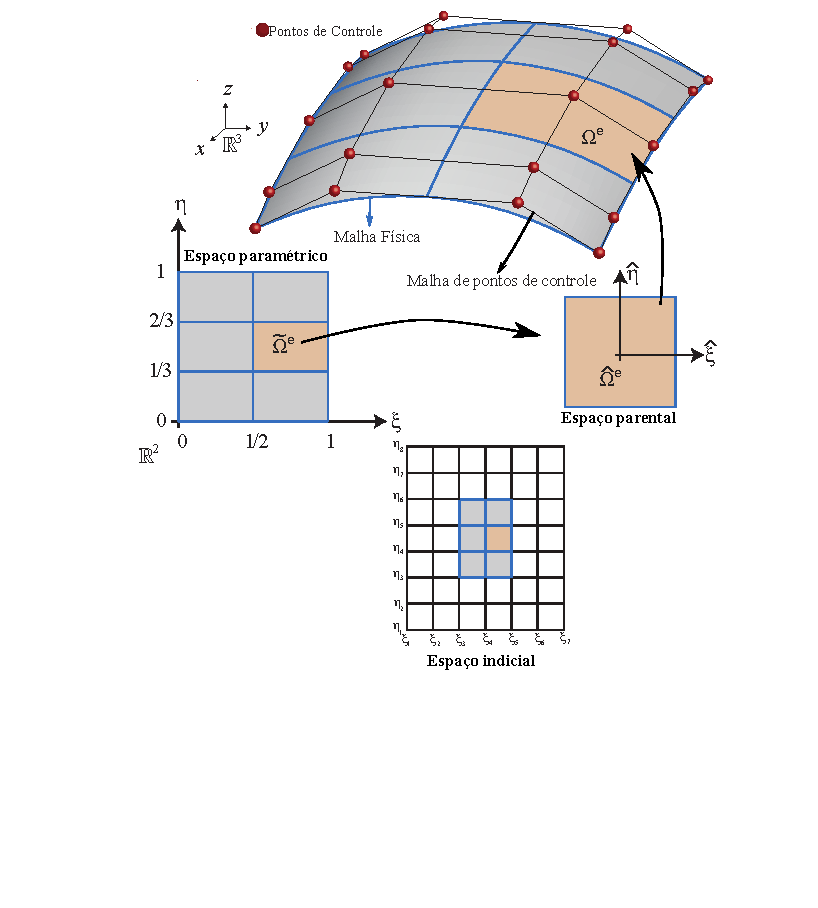
\includegraphics[scale=1.0,trim=1cm 4cm 0cm 0cm, clip=true]{Imagens/Cap2/espacosNURBS.pdf}	
	\caption{NURBS: espaço paramétrico, espaço indicial, espaço parental, malha de pontos de controle e malha física. Fonte: Adaptado de \citeonline{CottrelHB:2009}}
	\label{fig:espacos}
\end{figure}


A malha física representa a geometria discretizada, e dentro da malha física podem ainda ser definidos dois tipos de elementos, um macro-elemento, denominado de \textit{patch}, e o \textit{knot span}, que é o equivalente a um elemento finito e será denominado célula ao longo deste texto. Cada \textit{patch} é composto por um conjunto de células. Muitas geometrias simples podem ser discretizadas apenas com um \textit{patch}, entretanto, a depender da complexidade da mesma, se torna necessário o uso de um conjunto de \textit{patches}. As células são representações geométricas de linhas, superfícies e volumes nos espaços físicos unidimensional, bidimensional e tridimensional respectivamente.

Cada \textit{patch} e suas respectivas células possuem uma representação ainda no espaço paramétrico, que é o espaço onde as funções base são definidas. O espaço paramétrico, para os casos unidimensionais, é definido por um \textit{knot vector}, aqui denominado de vetor de \textit{knots}, que é um conjunto de coordenadas paramétricas. As células são constituídos pelo espaço entre duas coordenadas paramétricas ou dois \textit{knots}. O espaço onde se representam todos as células ou \textit{knot spans}, inclusive os nulos (quando mais de um \textit{knot} ocupa a mesma posição), é chamado de espaço indicial.

Por fim, na análise isogeométrica conta-se ainda com o espaço parental, que é o espaço de integração numérica das funções base, em geral, definido de forma adimensional de -1 a 1 dentro de uma célula. Na Fig. \ref{fig:espacos} pode-se observar os espaços relatados para uma superfície 3D construída por funções base quadráticas e apenas um \textit{patch}. 



\section{Re\-pre\-sen\-ta\-ção ge\-o\-mé\-tri\-ca u\-ti\-li\-zan\-do \newline{NURBS}}

\subsection{Vetor de \textit{knots}}

As funções \textit{B-Splines}, que são utilizadas na construção das NURBS, são definidas em um espaço paramétrico que é comum a um conjunto de células ou \textit{patch}. Um vetor de \textit{knots} em uma dimensão é um conjunto não decrescente de coordenadas no espaço paramétrico definido como: $\Xi=\left[\xi_{0},\xi_{1},...,\xi_{n+p+1}\right]$,  com $\xi_{i}\in \realspace$ representando a coordenada paramétrica do \textit{knot} $i$, $n$ é o número de funções base na direção paramétrica e $p$ o grau das mesmas.

Um \textit{knot} pode possuir multiplicidade maior do que um, e esse fato, implica em importantes mudanças nas funções base, que serão tratadas posteriormente. Os vetores de \textit{knots} conhecidos como abertos, são frequentemente utilizados nas literaturas de CAD, e caracterizam-se por ter a primeira e a última coordenada paramétrica repetidas $p+1$ vezes. Este fato garante que as funções unidirecionais sejam interpolatórias nos extremos do espaço paramétrico, proporcionando por exemplo a homogeneidade com respeito às condições de contorno essenciais. 

\subsection{\textit{B-Splines}}

As funções \textit{B-Splines} são definidas a partir de um vetor de \textit{knots}.  As funções podem ser obtidas recursivamente, sendo que para $p=0$ são escritas através da seguinte relação:

\begin{align}
N_{i,0}(\xi) = \begin{cases} 1 &\mbox{if } \xi_i\leq\xi<\xi_{i+1} \\
0 & \mbox{caso contrário } \end{cases},
\end{align}

\noindent enquanto que para funções com $p\geq1$ são definidas como:

\begin{align}
N_{i,p}(\xi)=\frac{\xi-\xi_{i}}{\xi_{i+p}-\xi_{i}}N_{i,p-1}(\xi) + 
\frac{\xi_{i+p+1}-\xi}{\xi_{i+p+1}-\xi_{i+1}}N_{i+1,p-1}(\xi).
\end{align}

Na Fig.\ref{fig:b-splines}, pode-se observar funções \textit{B-Splines} quadráticas construídas sobre o vetor de \textit{Knots} aberto $\Xi=\left[0,0,0,1,2,3,3,4,4,4\right]$. Pode-se observar que, devido à repetição dos \textit{Knots}  $p+1$ vezes nos extremos do vetor de \textit{knots}, as funções são interpoladoras nesses pontos, por outro lado a base passa a ser não uniforme. Além disso, devido o $knot$ $\xi = 3$ ter multiplicidade igual a 2, nota-se a perda da ordem de continuidade da função de forma nessa coordenada, passando a não apresentar derivada contínua sobre o \textit{knot}. A regra geral para a determinação da continuidade das funções é definida então como o grau das função ($p$) menos o número de vezes que uma coordenada paramétrica se repete.

\begin{figure}[htb!]
	\centering 
	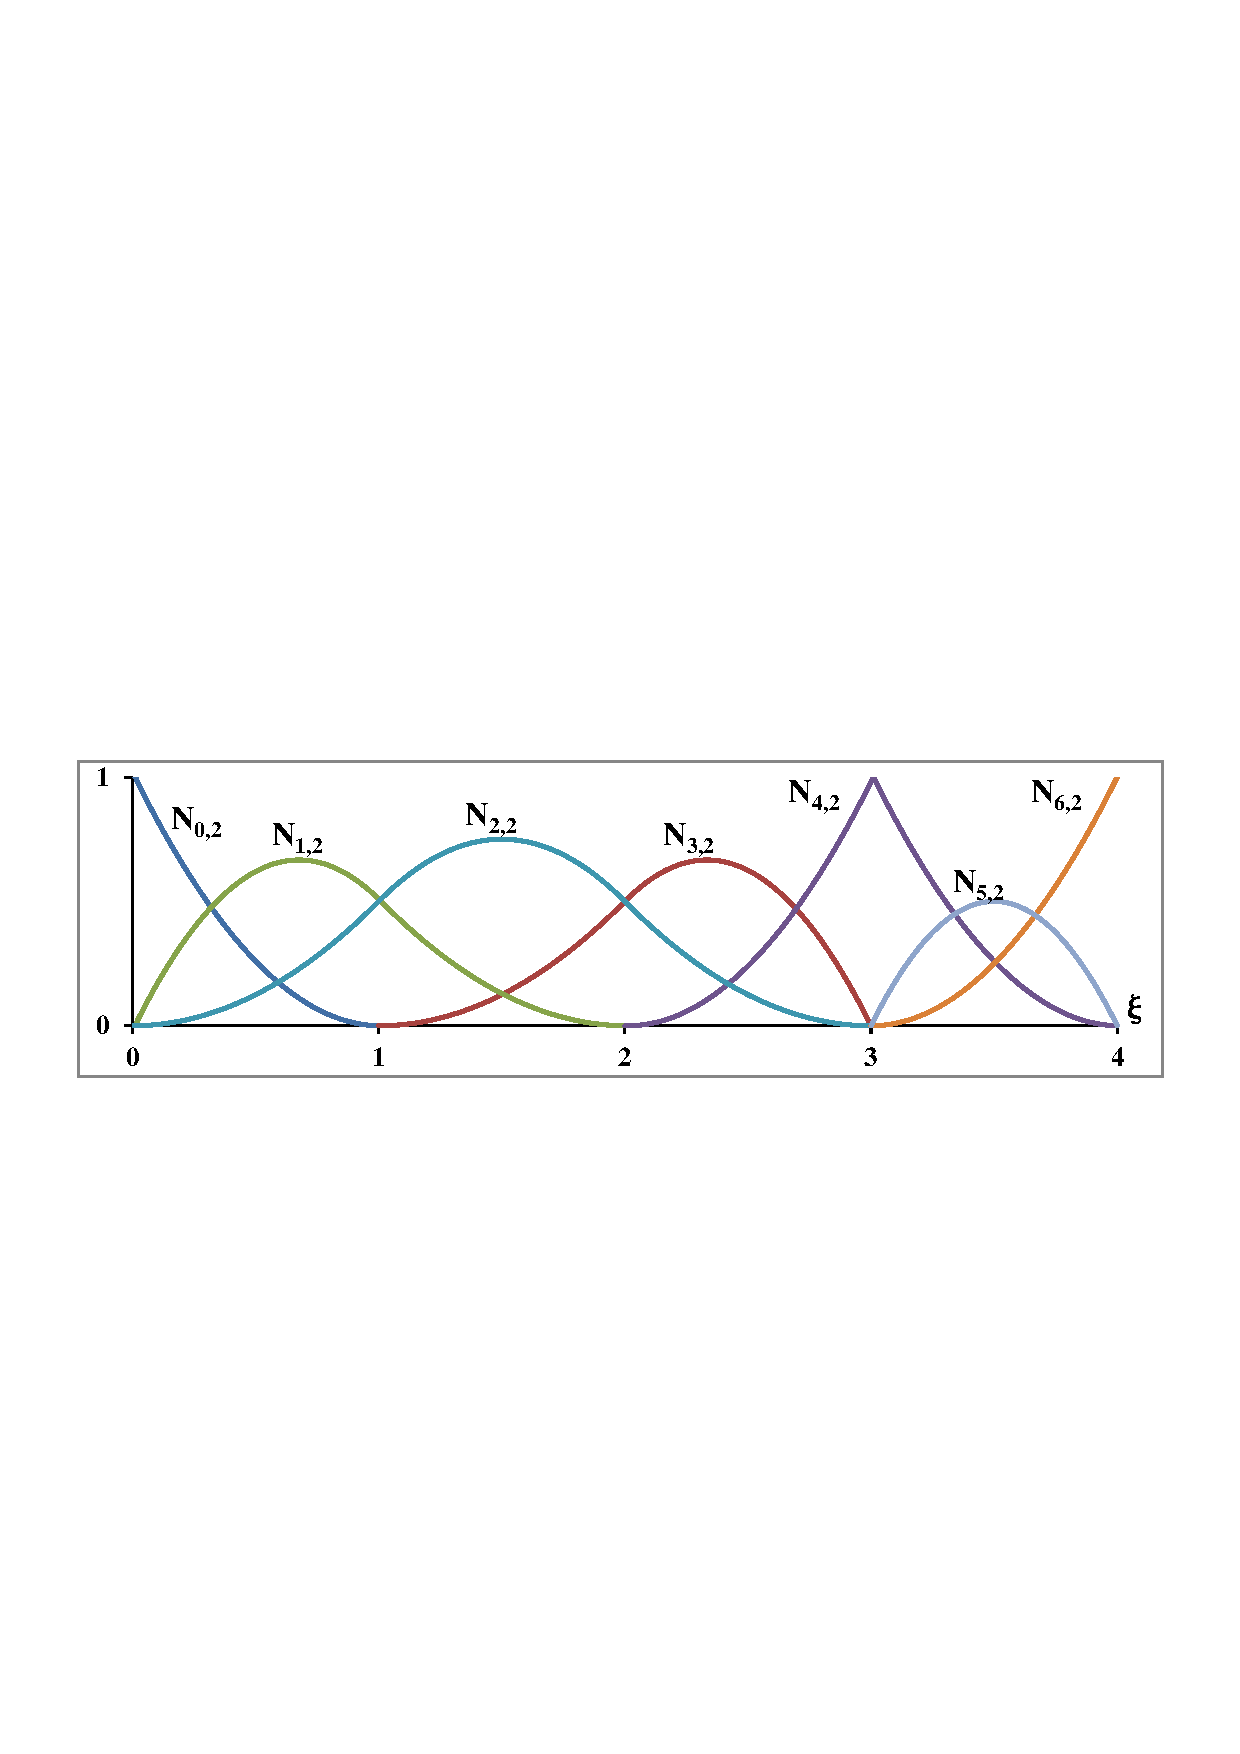
\includegraphics[scale=0.7,trim=0cm 11cm 0cm 12cm, clip=true]{Imagens/Cap2/B-splines1.pdf}	
	\caption{\textit{B-Splines}}
	\label{fig:b-splines}
\end{figure}

As principais propriedades das funções \textit{B-Splines} são:

\begin{itemize}
	\item \textbf{Partição da Unidade}: $\sum_{i=0}^{n}N_{i,p}(\xi)=1 $;
	\item \textbf{Positividade}: Todas as funções base são positivas, ou seja, $N_{i,p}\geq0$, $\forall\xi$;
	\item \textbf{Suavidade}: função de ordem $p$ é, em geral, $p-1$ vezes continua no contorno das células;
	\item \textbf{Suporte Compacto}: O suporte de cada $N_{i,p}$ está contido no intervalo $\left[\xi_i,\xi_{i+p+1}\right]$, ou seja, em cada célula, apenas $p+1$ funções são não nulas. % Deve-se notar no entanto que, ao se extenderem por vários elementos, o suporte é menos compacto do que para bases formadas por polinômios de lagrange definidos em elementos finitos.
\end{itemize}

A derivada de uma função de forma \textit{B-Spline} é calculada de acordo com a seguinte equação recursiva:

\begin{align}
N_{i,p}^d = p\left(\frac{N_{i,p-1}^{(d-1)}}{\xi_{i+p} - \xi_{i}} - \frac{N_{i+1,p-1}^{(d-1)}}{\xi_{i+p+1} - \xi_{i+1}}\right),
\end{align}

\noindent sendo $d$ a d-ésima derivada da função $N_{i,p}$.

Uma curva \textit{B-Spline} é construída a partir da combinação linear entre funções base e um conjunto de pontos de controle. Considerando um conjunto de $n$ funções base, $N_{i,p}$, com $i = 0,1,...,n$ e pontos de controle $\CP_i$ $\in \realspace$ e $i = 0,1,...,n$, uma curva polinomial por partes \textit{B-Spline} unidimensional é definida como:

\begin{align}
\mathbf{C} =\pos\left(\xi\right) = \sum_{i=0}^{n}N_{i,p}(\xi)\CP_i,
\end{align}

\noindent com $x$, $y$ e $z$ sendo as coordenadas físicas de um espaço cartesiano. Utilizando as funções \textit{B-Splines} apresentadas na Fig.\ref{fig:b-splines} e uma malha de pontos de controle qualquer, obtém-se a curva apresentada na Fig.\ref{fig:curva1}. Na Fig.\ref{fig:curva2} pode-se observar as células físicas equivalentes a essa combinação.

\begin{figure}[!htb]
	\centering	
	\subfloat[Malha de pontos de controle.\label{fig:curva1}]{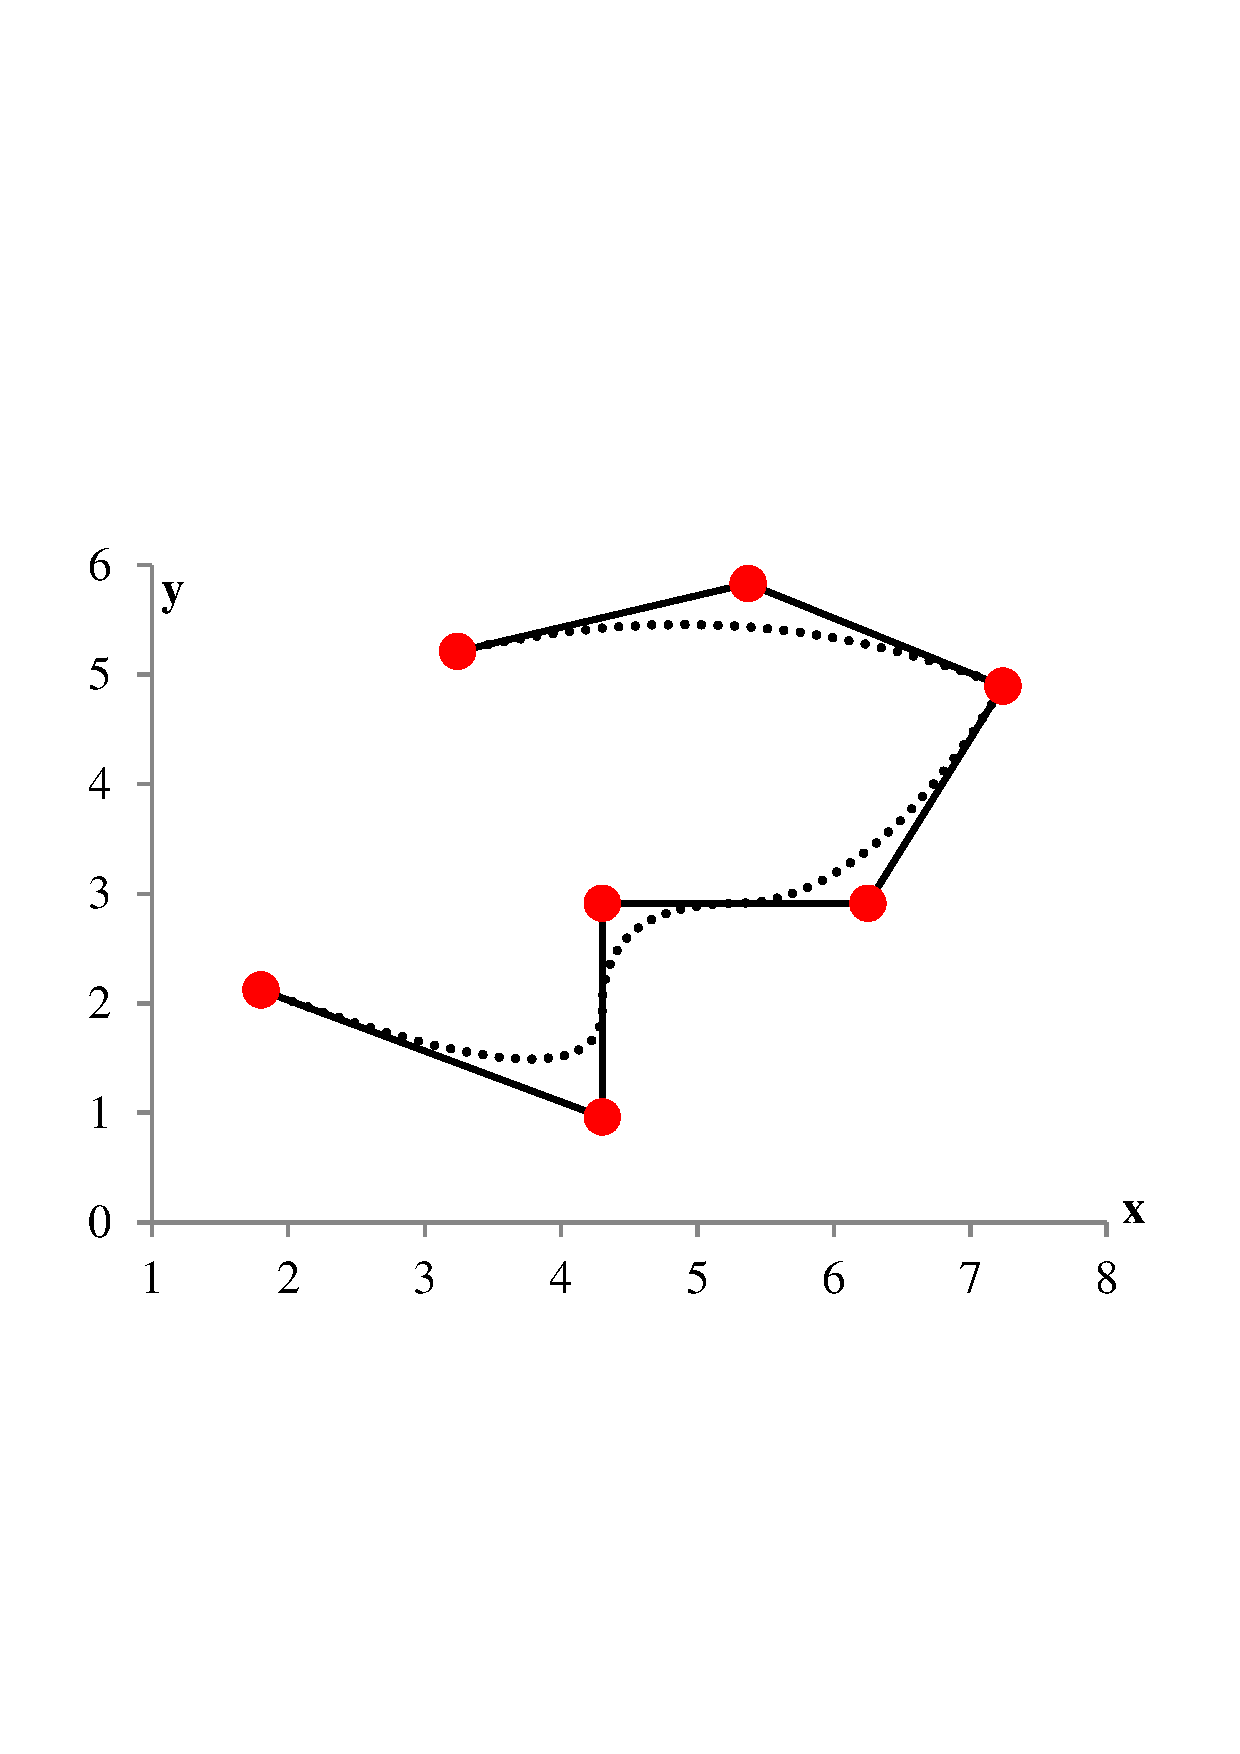
\includegraphics[scale=0.4,trim=1cm 7cm 1cm 9cm, clip=true]{Imagens/Cap2/B-splines2.pdf}}
	\subfloat[Representação física das células. \label{fig:curva2}]{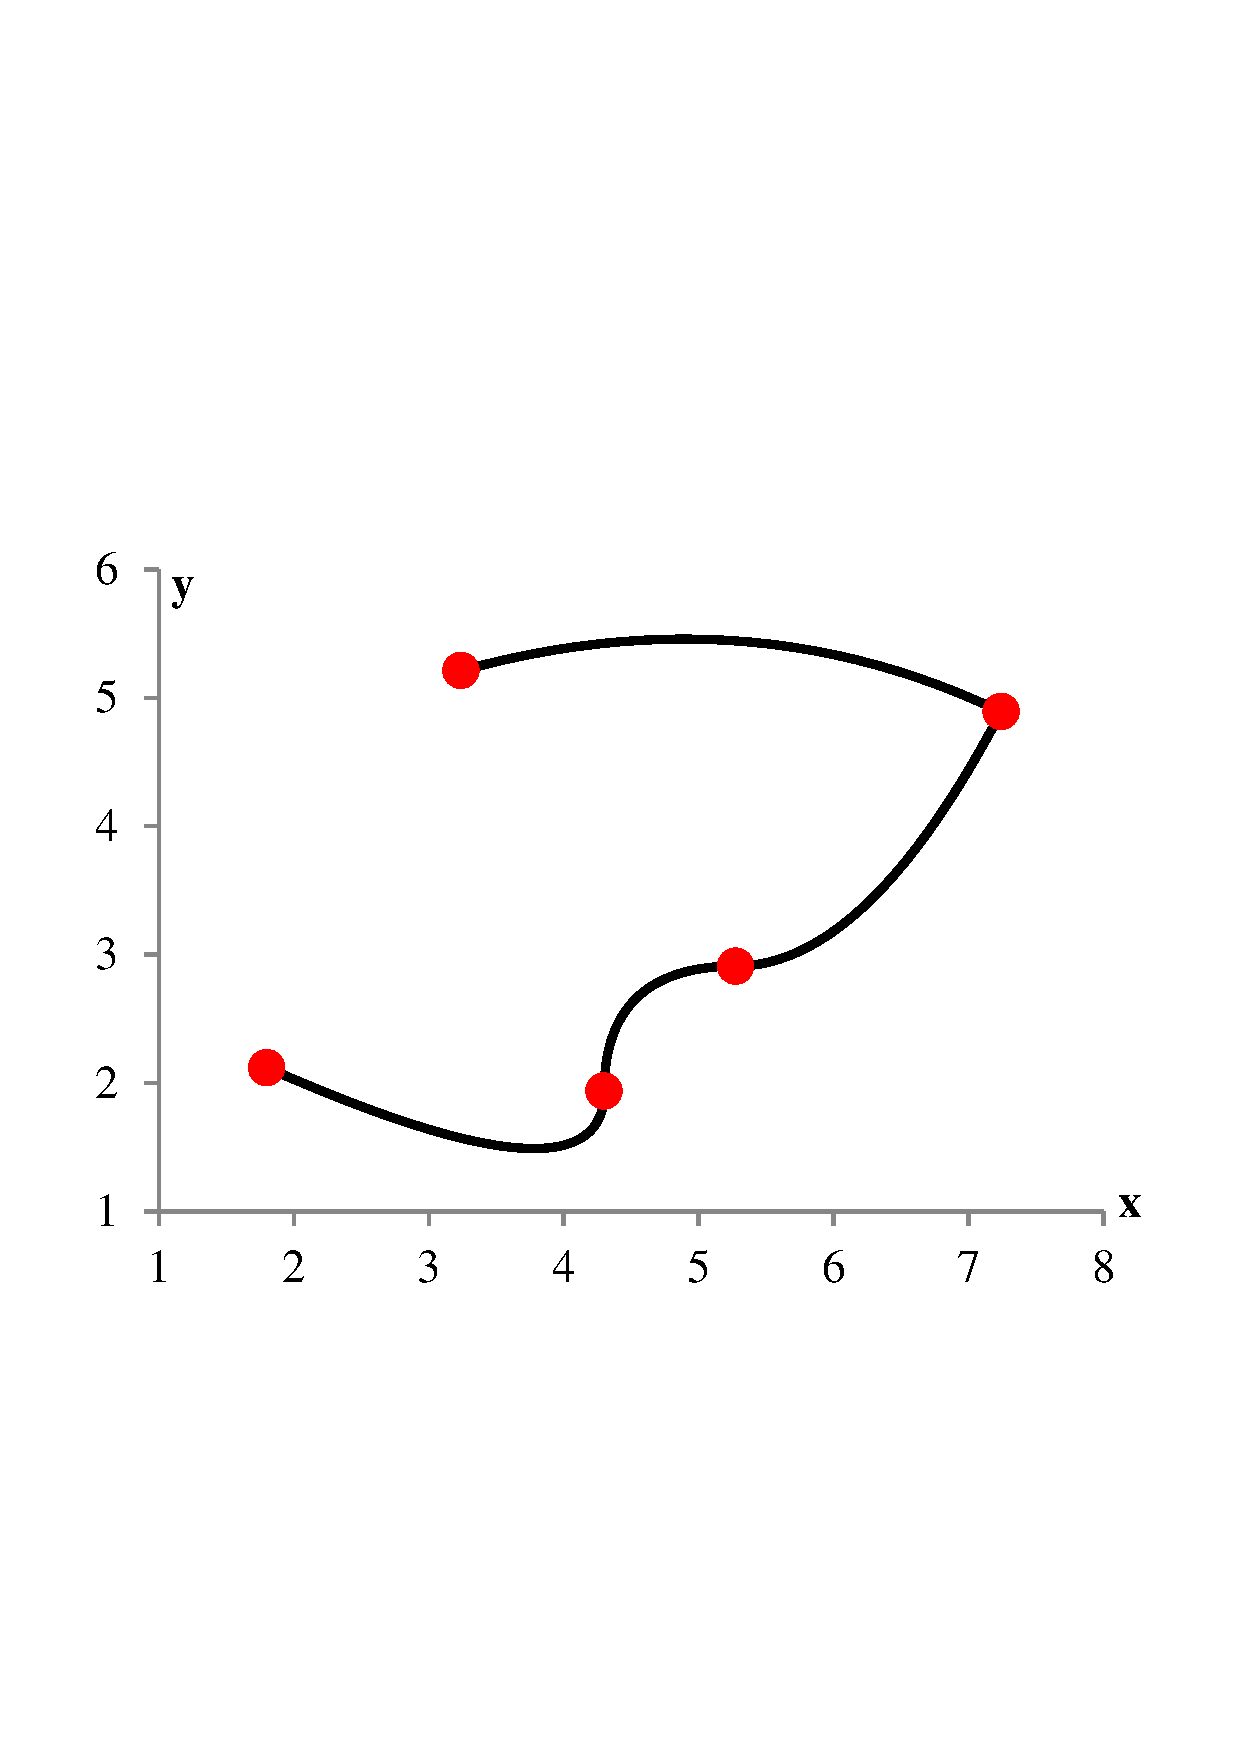
\includegraphics[scale=0.4,trim=1cm 7cm 1cm 9cm, clip=true]{Imagens/Cap2/B-splines3.pdf}}
	\caption{Curva \textit{B-Spline}}
\end{figure}

A partir da Fig.\ref{fig:curva1} pode-se constatar que a curva \textit{B-Spline} interpola o primeiro e o último ponto de controle, que é uma característica das curvas construídas com funções descritas a partir de vetores de nós abertos. Adicionalmente nota-se que, devido à multiplicidade do \textit{knot} de coordenada paramétrica $3$, existe um ponto de controle intermediário também interpolando a curva. Coordenadas paramétricas com multiplicidade igual ou superior ao grau do polinômio $p$ resultam em pontos de controle interpoladores. Por fim, observa-se ainda, que a multiplicidade de $\xi = 3$ resultou na perda da ordem de continuidade da curva sobre esse ponto, que passa a não ter derivada contínua.

Conforme observado  Fig.\ref{fig:curva1}, muitas das características das curvas \textit{B-Splines} são consequências das propriedades das funções \textit{B-splines}. Outra importante propriedade dessas curvas é a \textit{Transformação Afim}, significando que uma transformação na curva é obtida  se aplicarmos uma transformação afim aos pontos de controle. Devido ao suporte compacto das funções base, as curvas \textit{B-Splines} possuem característica denominada de \textit{localidade}, que significa que, movendo-se um ponto de controle, afeta-se não mais do que $p+1$ células na curva.

Uma superfície \textit{B-spline} é obtida analogamente. Dado uma rede de pontos de controle $\CP_{i,j}$, com $i = 0,1,...,n$ e $j = 0,1,..., m$, e vetores de \textit{knots} $\Xi = \left[\xi_{0},\xi_{1},...,\xi_{p+n+1}\right]$, $\mathcal{H} = \left[\eta_{0},\eta_{1},...,\eta_{q+m+1}\right]$, a superfície é obtida através do produto tensorial entre $n$ funções unidirecionais $N_{i,p}$ e $m$ funções unidirecionais $M_{j,q}$ da seguinte forma:

\begin{align}
\mathbf{S} = \pos\left(\xi,\eta\right)  = \sum_{i=0}^{n}\sum_{j=0}^{m}N_{i,p}(\xi)M_{j,q}(\eta)\CP_{i,j},
\end{align}

\noindent onde $q$ representa o grau das funções na direção paramétrica $\eta$. Devido à natureza do produto tensorial, as superfícies \textit{B-Splines} herdam as características citadas anteriormente para as curvas, sendo o suporte, por exemplo, de uma função bivariada $\hat{N}_{i,j:p,q}\left(\xi,\eta\right) = N_{i,p}(\xi)M_{j,q}(\eta)$ equivalente à: $\left[\xi_{i},\xi_{i+p+1}\right]\times\left[\eta_{j},\eta_{j+q+1}\right]$

Por fim, um sólido \textit{B-Splines} é obtido através do produto tensorial entre funções unidirecionais $N_{i,p}$, $M_{j,q}$, $L_{k,r}$, construídas sobre os vetores de \textit{knots} $\Xi = \left[\xi_{0},\xi_{1},...,\xi_{p+n+1}\right]$, $\mathcal{H} = \left[\eta_{0},\eta_{1},...,\eta_{q+m+1}\right]$ e $\mathcal{Z} = \left[\zeta_{0},\zeta_{1},...,\zeta_{l+r+1}\right]$ respectivamente, e um conjunto de pontos de controle  $\CP_{i,j,k}$ com $i = 0,1,...,n$, $j = 0,1,..., m$, $k = 0,1,..., m$, da seguinte forma:

\begin{align}
\mathbf{T} = \pos\left(\xi,\eta,\zeta\right)  = \sum_{i=0}^{n}\sum_{j=0}^{m}\sum_{k=0}^{l}N_{i,p}(\xi)M_{j,q}(\eta)L_{k,r}(\zeta)\CP_{i,j,k},
\end{align}

\noindent na qual $l$ e $r$ representam o número de funções e o grau das funções na direção paramétrica $\zeta$. Um sólido \textit{B-Spline} herda as características das respectivas curvas que o deram origem. Além disso, o suporte de uma função trivariada $\hat{N}_{i,j,k:p,q,r}\left(\xi,\eta,\zeta\right) = N_{i,p}(\xi)M_{j,q}(\eta)L_{k,r}(\zeta)$ está contido no intervalo $\left[\xi_{i},\xi_{i+p+1}\right]\times\left[\eta_{j},\eta_{j+q+1}\right]\times\left[\zeta_{k},\zeta_{k+r+1}\right]$.


\subsection{\textit{B-Splines} não-uniformes racionais e análise isogeométrica}

Uma entidade NURBS no $\realspace^{d}$ pode ser entendida, de ponto de vista geométrico, como a projeção transformativa de uma entidade \textit{B-Spline} no $\realspace^{d+1}$. Geometrias cônicas podem ser construídas exatamente pela projeção transformativa de curvas por partes quadráticas (para maiores detalhes sobre projeção transformativa, ver \citeonline{Farin:1999}). Na Fig. \ref{fig:circunferencia}, apresenta-se uma curva NURBS $\mathbf{C}\left(\xi\right)$, que representa, de forma exata, uma circunferência, sendo essa obtida a partir da projeção de uma curva \textit{B-Spline} $\mathbf{C}^{w}\left(\xi\right)$.

\begin{figure}[htb!]
	\centering 
	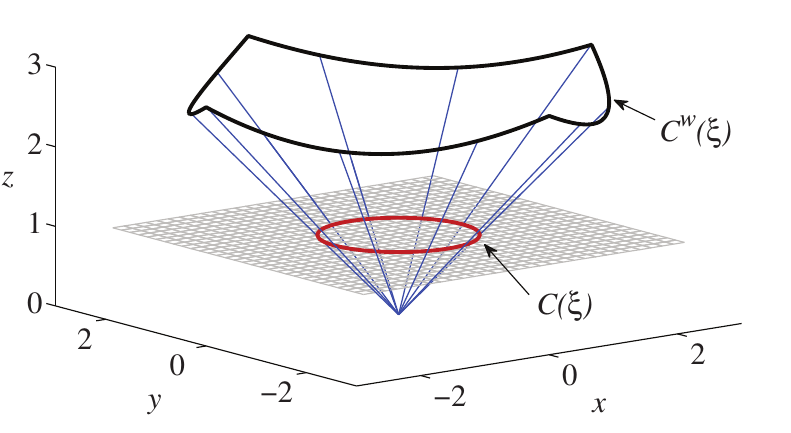
\includegraphics[scale=0.3,trim=0cm 0cm 0cm 0cm, clip=true]{Imagens/Cap2/transformacaoprojetiva.png}	
	\caption{Projeção transformativa para obtenção circunferência. Fonte: \citeonline{CottrelHB:2009}}
	\label{fig:circunferencia}
\end{figure}

Matematicamente, uma função NURBS é obtida pela racionalização de uma função \textit{B-Spline}. A racionalização dessa função ocorre através da razão entre dois polinômios. Uma função racional NURBS $\left(R\right)$ é construída através da seguinte expressão:

\begin{align}
R_{i}^{p}(\xi) = \frac{N_{i,p}(\xi)w_i}{\sum_{\hat{i}=0}^{n}N_{\hat{i},p}(\xi)w_{\hat{i}}}
\end{align}

\noindent onde $w_i$ e $w_{\hat{i}}$ $\in \realspace$, com $i = \hat{i} =  0, 1, ... , n$ , correspondem aos pesos relativos as funções $N_{i,p}\left(\xi\right)$ e $N_{\hat{i},p}\left(\xi\right)$ respectivamente. 

A $d$-ésima derivada de $R_{i}$ (onde suprimiu-se o índice $p$ para facilitar a representação), é obtida da seguinte forma:

\begin{align}
R_{i}^{d}(\xi) = \frac{N_{i}^{d}(\xi)w_i - \sum_{l=1}^{d}\left[\binom{d}{l}\sum_{j=1}^{n}N_{j}^{l}(\xi)w_{j}R_{i}^{d-l}(\xi)\right]}{\sum_{{j}=0}^{n}N_{{j}}(\xi)w_{{j}}},
\end{align}

\noindent em que:
\begin{align}
\binom{d}{l} = \frac{d!}{l!\left(d-l\right)!}.
\end{align}

Uma curva NURBS é obtida por:

\begin{align}
\mathbf{C} = \pos\left(\xi\right) = \sum_{i=0}^{n}R_{i}^{p}(\xi)\CP_i, \label{eq:curveNURBS}
\end{align}

\noindent sendo os pesos selecionados de maneira a se obter a geometria desejada. Analogamente uma superfície NURBS é obtida através das seguintes relações:

\begin{align}
R_{i,j}^{p,q}(\xi,\eta) = \frac{N_{i,p}(\xi)M_{j,q}(\eta)w_{i,j}}{\sum_{\hat{i}=0}^{n}\sum_{\hat{j}=0}^{m}N_{\hat{i},p}(\xi)M_{\hat{j},q}(\eta)w_{\hat{i},\hat{j}}},
\end{align}

\begin{align}
\mathbf{S} = \pos\left(\xi,\eta\right) = \sum_{i=0}^{n}\sum_{j=0}^{m}R_{i,j}^{p,q}(\xi,\eta)\CP_{i,j}, \label{eq:surfaceNURBS}
\end{align}

\noindent com $w_{i,j}$ e $w_{\hat{i},\hat{j}}$ $\in \realspace$, sendo $i = \hat{i} =  0, 1, ... , n$ e  $j = \hat{j} =  0, 1, ... , m$ , correspondem aos pesos relativos às funções $\left(N_{i,p}\left(\xi\right)M_{j,q}\left(\eta\right)\right)$ e $\left(N_{\hat{i},p}\left(\xi\right)M_{\hat{j},q}\left(\eta\right)\right)$ respectivamente. Por fim, um sólido NURBS é obtido por:

\begin{align}
R_{i,j,k}^{p,q,r}(\xi,\eta,\zeta) = \frac{N_{i,p}(\xi)M_{j,q}(\eta)L_{k,r}(\zeta)w_{i,j,k}}
{\sum_{\hat{i}=0}^{n}\sum_{\hat{j}=0}^{m}\sum_{\hat{k}=0}^{l}N_{\hat{i},p}(\xi)M_{\hat{j},q}(\eta)L_{\hat{k},r}(\zeta)w_{\hat{i},\hat{j},\hat{k}}},
\end{align}

\begin{align}
\mathbf{T} = \pos\left(\xi,\eta,\zeta\right) = \sum_{i=0}^{n}\sum_{j=0}^{m}\sum_{k=0}^{l}R_{i,j,k}^{p,q,r}(\xi,\eta,\zeta)\CP_{i,j,k}, \label{eq:solidNURBS}
\end{align}

\noindent onde $w_{i,j,k}$ e $w_{\hat{i},\hat{j},\hat{k}}$ $\in \realspace$, sendo $i = \hat{i} =  0, 1, ... , n$, $j = \hat{j} =  0, 1, ... , m$ e $k = \hat{k} =  0, 1, ... , l$, correspondem aos pesos relativos às funções $\left(N_{i,p}\left(\xi\right)M_{j,q}\left(\eta\right)L_{k,r}\left(\zeta\right)\right)$ e $(N_{\hat{i},p}\left(\xi\right)M_{\hat{j},q}\left(\eta\right)L_{\hat{k},r}\left(\zeta\right))$ respectivamente.

Na aplicação da IGA, as funções tentativa para velocidade e pressão, e as funções peso associadas a elas, apresentadas nas Eq. \eqref{eq:vel} à Eq. \eqref{eq:ptest} como $N$, são equivalentes à $R_{i}^{p}(\xi)$, $R_{i,j}^{p,q}(\xi,\eta)$ e $R_{i,j,k}^{p,q,r}(\xi,\eta,\zeta)$ para os casos unidimensional, bidimensional e tridimensional respectivamente. E a geometria é representada pelas Eq. \eqref{eq:curveNURBS}, Eq. \eqref{eq:surfaceNURBS} e Eq. \eqref{eq:solidNURBS} dependendo da dimensão do problema em análise. 

A integração numérica nas células é realizada através da quadratura Gaussiana. Considerando o domínio paramétrico de uma célula $\tilde{\domain}^{e}$ e o domínio parental $\hat{\domain}^{e}$  apresentados na Fig.\ref{fig:espacos}, definidos respectivamente em um espaço tridimensional pelas coordenadas $\coordAdimen\left(\xi,\eta,\zeta\right)$ e $\hat{\coordAdimen}(\hat{\xi},\hat{\eta},\hat{\zeta})$, a matriz jacobiana do mapeamento do espaço físico, com coordenadas $\mathbf{x} \left(x,y,z\right)$,  para o espaço de quadratura, é definida por:

\begin{align}
\frac{d\pos}{d\hat{\coordAdimen}} = \frac{d\pos}{d\coordAdimen} \frac{d\coordAdimen}{d\hat{\coordAdimen}} \label{eq:integ}
\end{align}

O primeiro termo à direita da igualdade da Eq. \eqref{eq:integ} é calculado a partir das derivadas de Eq. \eqref{eq:curveNURBS}, Eq. \eqref{eq:surfaceNURBS} e Eq. \eqref{eq:solidNURBS} e o segundo termo, considerando a célula $\tilde{\domain}^{e} = [\xi_{i},\xi_{i+1}] \times [\eta_{j},\eta_{j+1}] \times [\zeta_{k},\zeta_{k+1}]$, calcula-se $\xi,\eta, \zeta$ $\in \tilde{\domain}^{e}$ a partir de $\hat{\xi},\hat{\eta}, \hat{\zeta}$ $\in \hat{\domain}^{e}$ através das seguintes relações: 


\begin{align}
\xi = \xi_{i} + \left(\hat{\xi}+1\right) \left(\frac{\xi_{i+1}-\xi_{i}}{2}\right),
\end{align}

\begin{align}
\eta = \eta_{i} + \left(\hat{\eta}+1\right) \left(\frac{\eta_{i+1}-\eta_{i}}{2}\right)
\end{align}

\noindent e

\begin{align}
\zeta = \zeta_{i} + \left(\hat{\zeta}+1\right) \left(\frac{\zeta_{i+1}-\zeta_{i}}{2}\right).
\end{align}


\section{Verificação e aplicações}

Para aplicação da IGA em problemas da DFC seguiu-se o mesmo procedimento matemático descrito ao longo do Cap. \ref{capitulo:Cap1}, sendo que a implementação computacional seguiu o roteiro apresentado no Alg. \ref{alg:fluid_temporalIntegration}. Os exemplos escolhidos para a verificação do código computacional foram o escoamento sobre um cilindro 3D e o problema de escoamento sobre um canal com degrau utilizando células 3D. Os resultados obtidos são apresentados nas seções subsequentes.

\subsection {Escoamento sobre um cilindro - 3D}

Na geração da geometria NURBS, correspondente ao problema do escoamento sobre um cilindro, utilizou-se um código previamente desenvolvido pela estudante durante seu mestrado \cite{Tonon:2016}. Por tratar-se de uma geometria de pequena complexidade, pôde-se gerá-la com um único \textit{patch}, o qual é composto por um cubo com um cilindro inserido em seu centro.
O processo de geração da malha, simplificadamente, consiste em se escolher vetores de $knots$, pontos de controle, e pesos adequados para a descrição de tal geometria.

O código previamente desenvolvido, baseia-se na quantidade mínima de pontos de controle necessários para gerar uma circunferência completa (ver Fig. \ref{fig:pontosdecontroleInicias}). Para a obtenção exata de uma circunferência utilizam-se funções quadráticas e o vetor de \textit {knots} na direção paramétrica $\xi$ inicial é composto por: $\Xi=\left[0,0,0,1/4,1/4,1/2,1/2,3/4,3/4,1,1,1\right]$. A posição dos pontos de controle da circunferência e seus respectivos pesos foram obtidos de acordo com \citeonline {PiegT:1996}. 

A obtenção da curva respectiva ao quadrado, que é descrita no espaço paramétrico correspondente a direção $\xi$, é consequência das escolhas realizadas para gerar a circunferência, logo, a curva possui o mesmo vetor de \textit{knots} e funções quadráticas. Os pontos de controle para a formação do quadrado foram posicionados, no espaço físico, de forma a ser obtida a dimensão requerida à seção transversal quadrada que compõe a geometria do cubo, e de forma que os mesmos ficassem alinhados com os pontos de controle da circunferência na direção radial. Os pesos respectivos ao pontos de controle do retângulo são unitários. Na Fig. \ref{fig:pontosdecontroleInicias} pode-se observar a posição dos pontos de controle respectivos à circunferência e ao quadrado e as curvas resultantes desta discretização em linha vermelho pontilhado.

Na sequência o código realiza o procedimento de refinamento por inserção sucessiva de \textit{knots} no vetor de \textit{knots}. O algoritmo utilizado para este procedimento pode ser encontrado em \citeonline {PiegT:1996}. Na Fig. \ref{fig:pontosdecontroleInicias2} apresenta-se um exemplo de pontos de controle gerados após a inserção de um novo \textit{knot} no centro de cada \textit{knot span} do espaço paramétrico inicial. A quantidade de \textit{knots} a ser inserida depende da discretização necessária a análise numérica.

\begin{figure}[!htb]
	\centering	
	\subfloat[Pontos de controle inicias.\label{fig:pontosdecontroleInicias}]{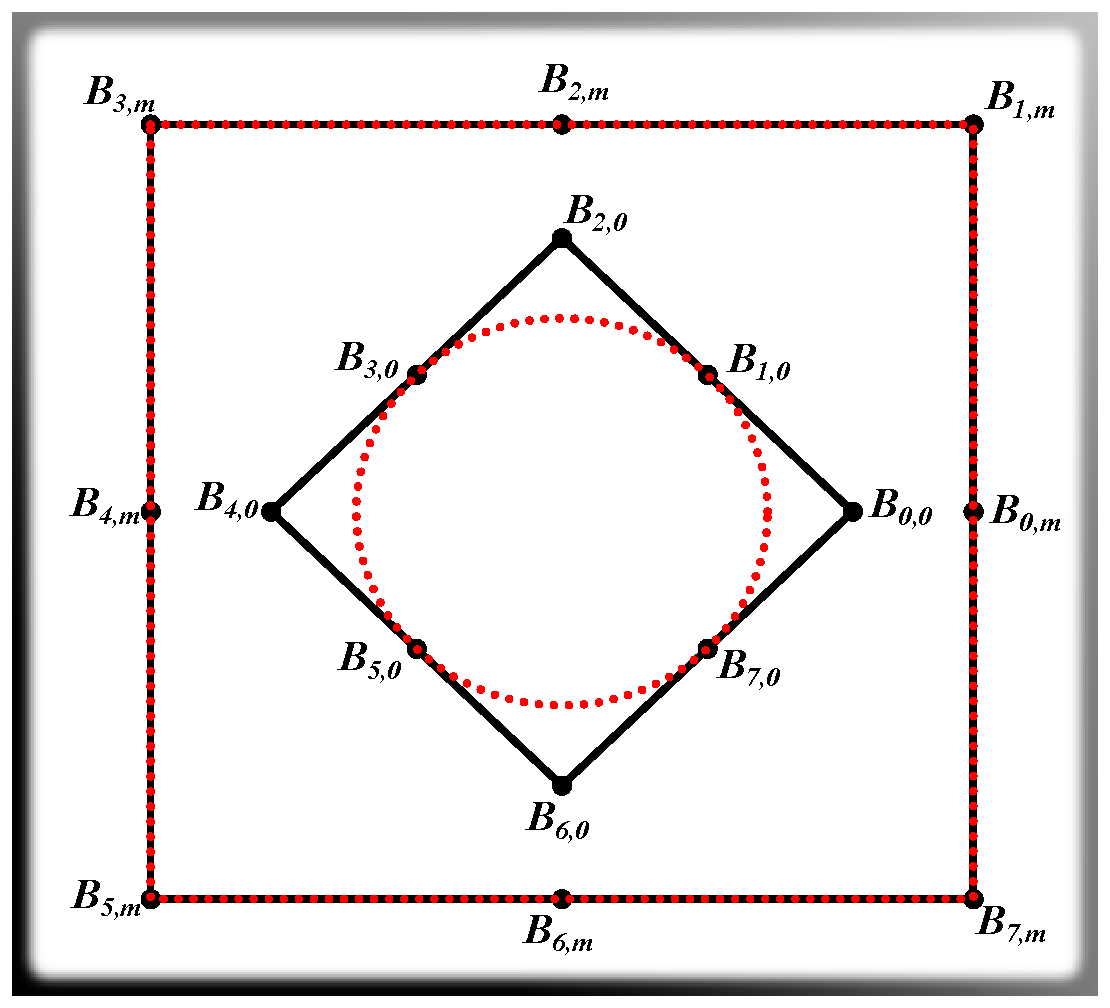
\includegraphics[scale=0.4,trim=1cm 1cm 0.5cm 1cm, clip=true]{Imagens/Cap2/escoamentosobrecilindro.pdf}}
	\subfloat[Pontos de controle após inserção de \textit{knots}.\label{fig:pontosdecontroleInicias2}]{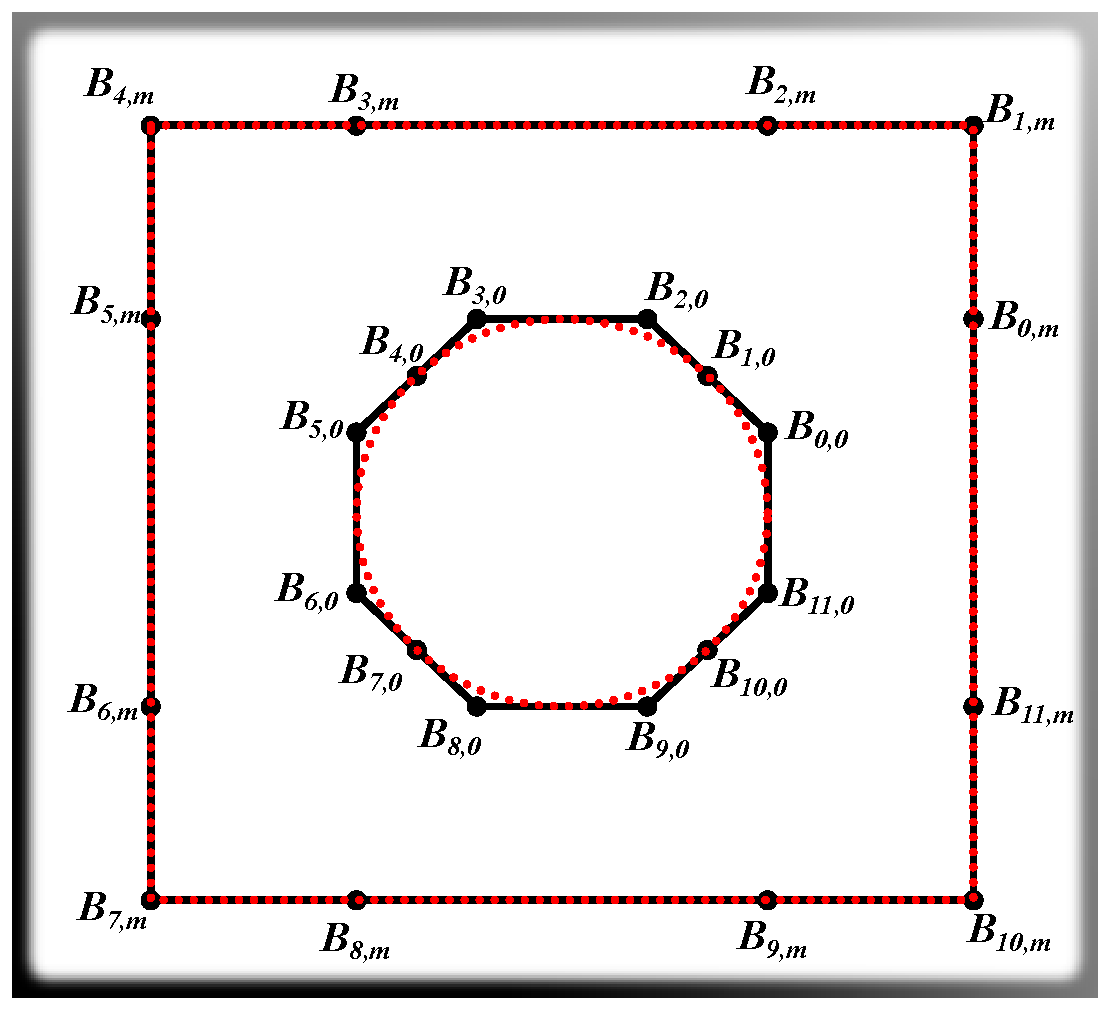
\includegraphics[trim=1cm 1cm 0.5cm 1cm,clip,scale=0.4]{Imagens/Cap2/escoamentosobrecilindro2.pdf}}
	\caption{Cilindro 3D: Geração curva NURBS}
\end{figure}

Para a obtenção de uma seção transversal da geometria em questão, gera-se uma superfície a partir da discretização na direção $\eta$ do espaço paramétrico. O código utiliza um vetor de \textit{knots} aberto, com os 
\textit{knots} distribuídos uniformemente, e funções de forma quadráticas. Os pontos de controle são distribuídos radialmente no espaço físico através de uma progressão geométrica unidirecional e seus pesos são determinados a partir de uma interpolação linear entre os pesos dos pontos de controle da circunferência e os pontos do quadrado. A quantidade mínima de pontos de controle respectiva à direção $\eta$ é de $q+1$ pontos, sendo a quantidade final definida em função da análise numérica. Na Fig. \ref{fig:superficieNURBcilindro}, apresenta-se um exemplo de uma rede de pontos de controle, obtida a partir das curvas apresentadas em Fig. \ref {fig:pontosdecontroleInicias2} com 9 pontos de controle na direção $\eta$. Na figura em questão omitiu-se a nomenclatura dos pontos de controle intermediários às curvas da circunferência e do quadrado para evitar a sobreposição da nomenclatura na figura.


\begin{figure}[htb!]
	\centering 
	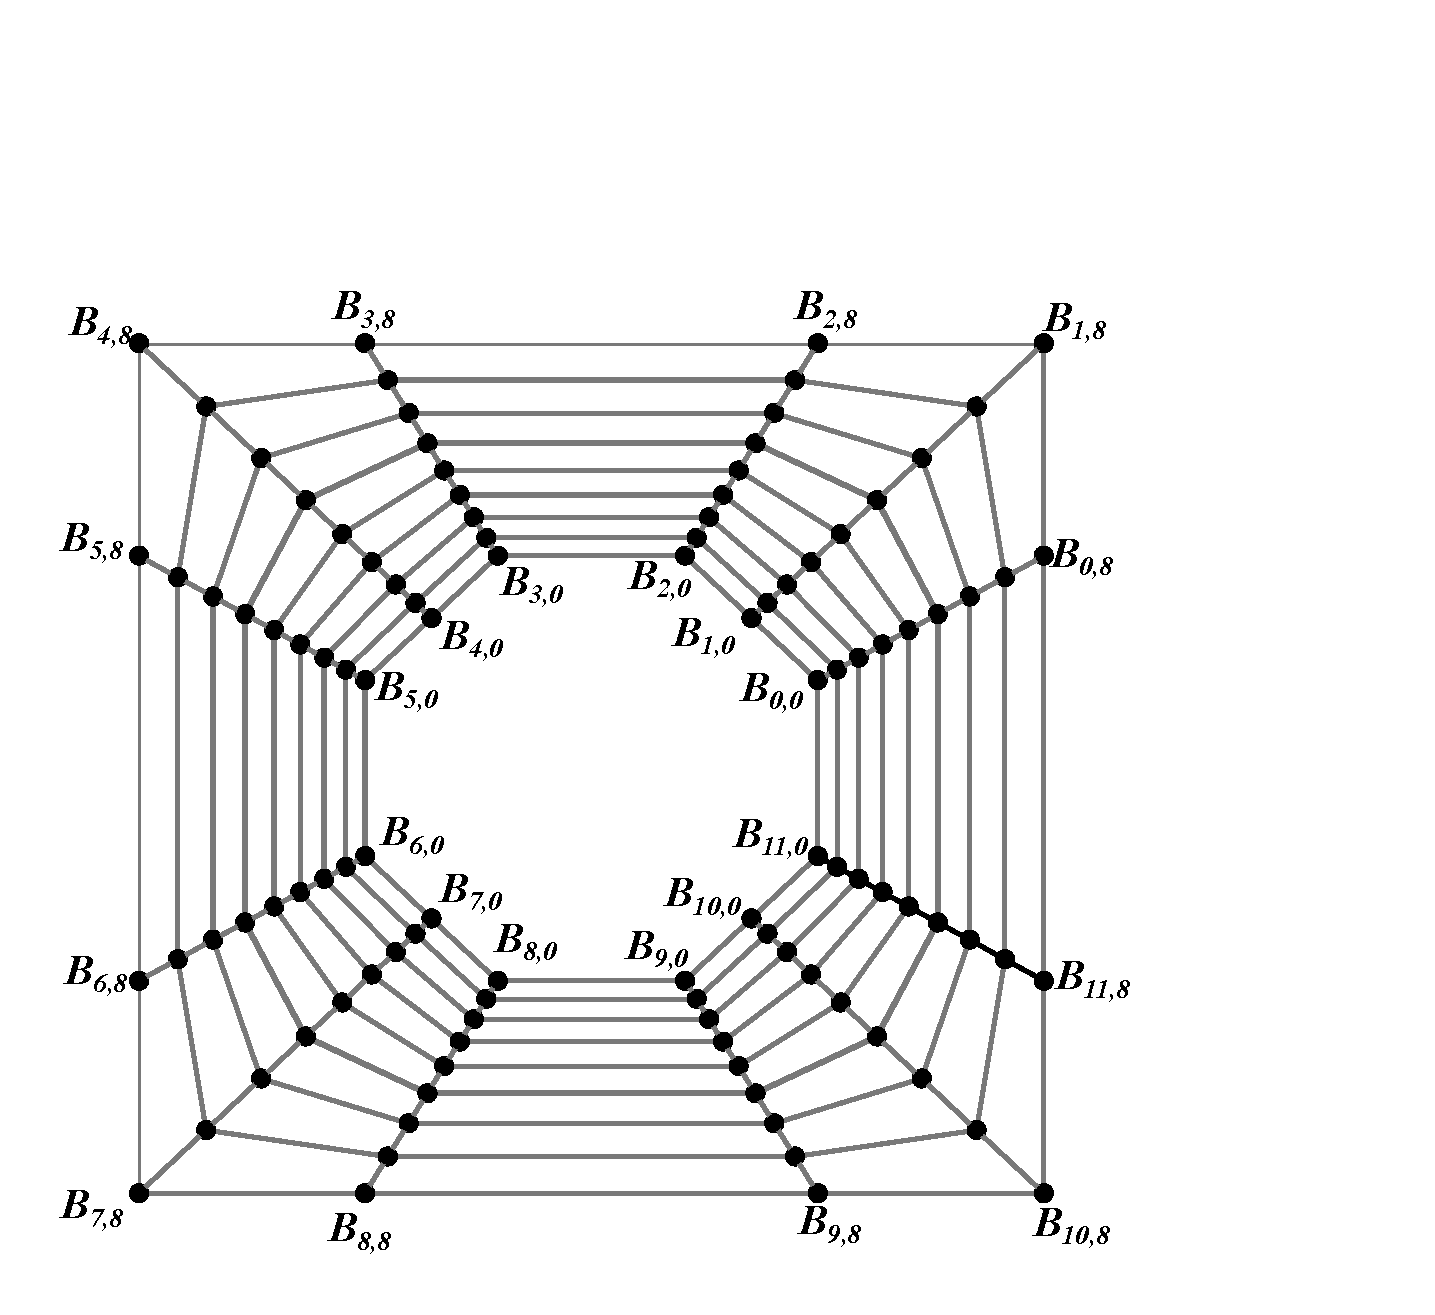
\includegraphics[scale=0.4,trim=1cm 1cm 5cm 4cm, clip=true]{Imagens/Cap2/escoamentosobrecilindro3.pdf}	
	\label{fig:superficieNURBcilindro}
	\caption{Cilindro 3D: Geração superfície NURBS.}
\end{figure}

Nessa primeira etapa do trabalho, a direção paramétrica $\zeta$, respectiva à direção $z$ da geometria física, foi discretizada com apenas uma célula, utilizando-se para isso vetor de \textit{knots} abertos com distribuição uniforme de \textit{knots}, e funções base quadráticas.

Visando a verificação do código de IGA 3D analisa-se o problema do escoamento sobre o cilindro para $\Reynolds$ =40 ,100 e 1000 (Eq. \eqref{eq:Reynolds}). Para isso, gera-se uma malha com 101 x 71 x 3 pontos de controle nas direções paramétricas $\xi$, $\eta$ e $\zeta$ respectivamente, resultando em 6624 células. Na Fig. \ref{fig:cilindrogeometria} apresentam-se as dimensões da geometria em questão, bem como as condições de contorno aplicadas, e na Fig. \ref{fig:cilindromalha} apresenta-se a malha física resultante da discretização.


\begin{figure}[!htb]
	\centering
	\subfloat[\label{fig:cilindrogeometria}Geometria]{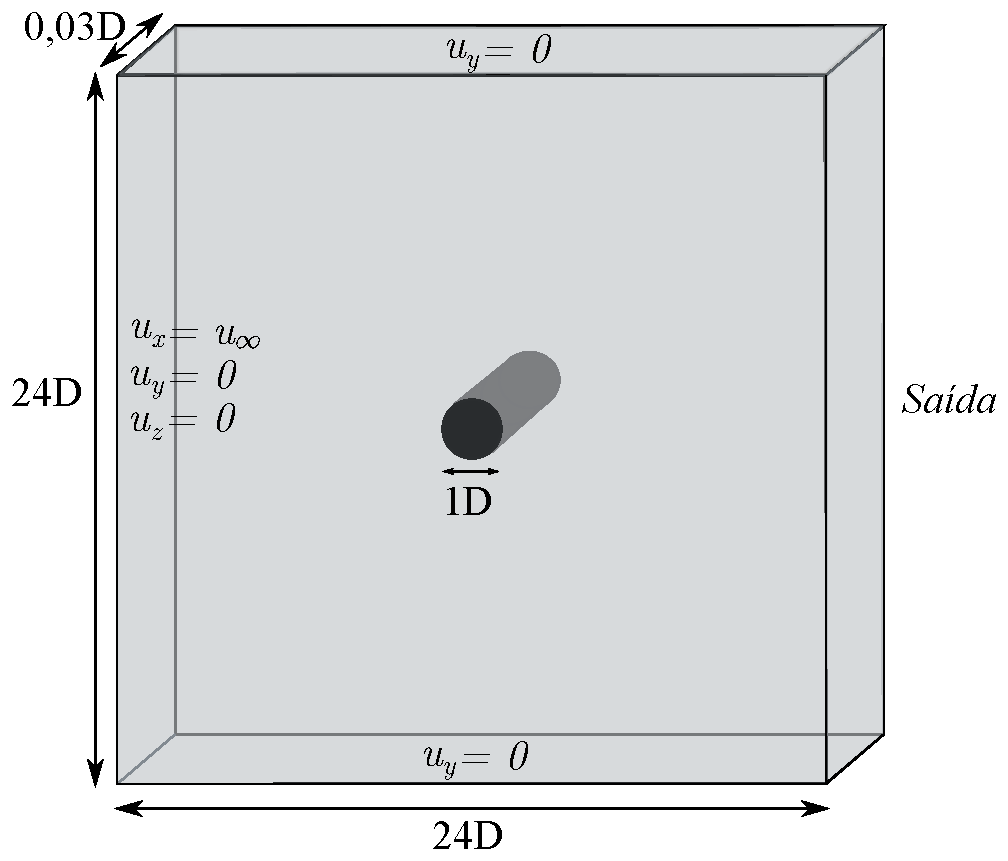
\includegraphics[scale=0.48,trim=0cm 0cm 0cm 0cm, clip=true]{Imagens/Cap2/cylinderISO3d.pdf}} 
	\subfloat[\label{fig:cilindromalha} Malha de células físicas]{\includegraphics[scale=0.2,trim=5cm 0cm 0cm 0cm, clip=true]{Imagens/Cap2/malhacilindro.eps}} 
	\caption{Cilindro 3D: Geometria e malha de células físicas}
	\label{fig:cilindro_geoemalha}
\end{figure}

Adicionalmente, prescrevem-se nas paredes frontal e posterior, condição de parede lisa ($u_{z} = 0$), e na \textit{Saída} do escoamento condição de força de superfície nula ($\stresstensor \normal = \mathbf{0}$). O problema é simulado para um velocidade de entrada $u_{\infty} = 1,0$, $\rho = 1,0$, $\timeStep = 0,05$, e $\specRadius = 0,5$, sendo a viscosidade variada de acordo com o número de Reynolds desejado.  Para o cálculo dos coeficientes aerodinâmicos $C_{D}$, $C_{L}$ e do número de Strouhal ($\Strouhal$) utilizam-se as equações apresentadas no Item \ref{subsection:escoamentocil2d}. 

Nas Figs. \ref{fig:cilindro_Cd3d} e \ref{fig:cilindro_Cl3d}, apresentam-se a variação ao longo do tempo dos coeficientes $C_{D}$ e $C_{L}$. Os valores obtidos com a malha isogeométrica 3D estão muito próximos ao obtidos com a malha de elementos finitos 2D (Item \ref{subsection:escoamentocil2d}) para Reynolds 40 e 100. Para Reynolds 1000, nota-se que a variação ao longo do tempo dos valores de $C_{D}$ e $C_{L}$ para IGA resulta em valores mais elevados do que os obtidos com MEF. Tal diferença ainda deverá ser investigada, sendo que tanto as diferenças nas dimensões das malhas como a diferença que pode haver na convergência dos resultados ou a efeitos de 3D de vorticidade podem contribuir para isso. Os resultados obtidos para o histórico de $C_{D}$ e $C_{L}$ por \citeonline{Henderson:1997} para $Re = 1000$ em análises tridimensionais baseadas em MEF, foram menores do que os 2D. Essa disparidade entre os resultados obtidos nesse trabalho e de \citeonline{Henderson:1997} podem estar relacionados com o fato de que a dimensão escolhida da malha na direção $z$ foi muito pequena de maneira a impossibilitar que os efeitos tridimensionais do escoamento fossem adequadamente capturados.

Para o número de Strouhal, o valor obtido para $\Reynolds = 100$ foi de 0,1681 e para $\Reynolds = 1000$ de 0,2395. Nota-se que, embora os valores de $C_{D}$ e $C_{L}$ apresentem diferenças entre os resultados 2d baseados em elementos finitos e a malha 3D baseada em IGA, a frequência do desprendimento de vórtices obtida foi muito semelhante.

\begin{figure}[!htb]
	\centering
	\subfloat[\label{fig:cilindro_Cd3d}Coeficiente de arrasto $ C_D$.]{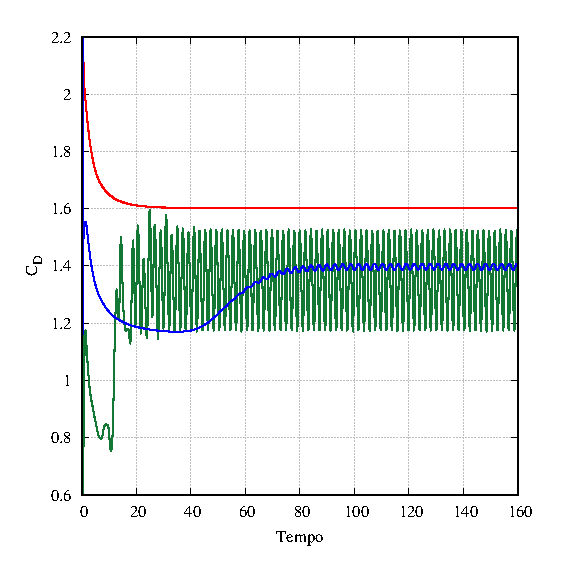
\includegraphics[scale=0.8,trim=0cm 0cm 0cm 0cm, clip=true]{Imagens/Cap2/DragRe.eps}} 
	\subfloat[\label{fig:cilindro_Cl3d}Coeficiente de sustentação $C_L$.]{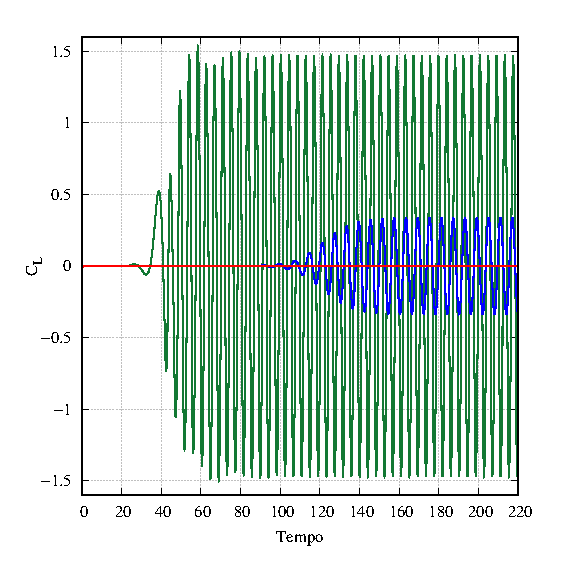
\includegraphics[scale=0.8,trim=0cm 0cm 0cm 0cm, clip=true]{Imagens/Cap2/LiftRe.eps}}\\ 
	{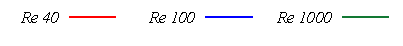
\includegraphics[scale=1.3]{Imagens/Cap2/Legenda.pdf}}
	\caption{Cilindro 3D: Coeficientes aerodinâmicos. }
	\label{fig:cilindro_coeficientes3d}
\end{figure}


\subsection {Escoamento em um canal com degrau}

Este exemplo é amplamento utilizado na verificação de códigos para escoamentos incompressíveis, sendo sua geometria apresentada na Fig. \ref{fig:degrau_geo}.  O problema consiste em prescrever-se um perfil parabólico de escoamento na entrada do canal, e condição de aderência ($\velocity = 0$) nas demais paredes que estão contidas nos planos $xz$ e $yz$, exceto na saída do canal, a qual possui como condição $\stresstensor\normal = \mathbf{0}$. Para as paredes dos planos $xy$, frontal e posterior, prescreveu-se condição de parede lisa ($u_{z}=0$). 

\begin{figure}[htb!]
	\centering
	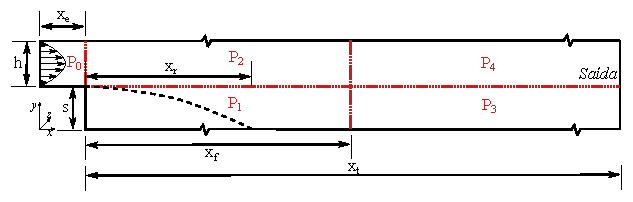
\includegraphics[scale=1.2,trim=0cm 0cm 0cm 0cm, clip=true]{Imagens/Cap2/degrau.pdf}
	\caption{Degrau 3D: Geometria.}
	\label{fig:degrau_geo}
\end{figure}


As dimensões selecionadas para o canal foram $h = 1,0m$, $s = 0,94m$, $x_{e}= 1,0m$, $x_{f}= 15m$ e $x_{t} = 30m$ e dimensão na direção $z$ de $0,1m$. Adicionalmente, o perfil de velocidade na entrada do canal é descrito pela seguinte relação:

\begin{align}
u_{x} = V_{max} \left(1-\left(\frac{\left(y-s\right)-h/2}{h/2}\right)^{2}\right),
\end{align}

\noindent com velocidade $V_{max} = 10 m/s$ e $u_{y} = u_{z} = 0$.

O escoamento sobre o degrau é caracterizado por produzir áreas de recirculação onde o fluido se separa e forma vórtices. A distância entre o degrau e o ponto de recolamento do vórtice principal $x_{r}$ é uma das principais características verificadas nesse problema. A dimensão dos vórtices varia em função do número de $\Reynolds$, a qual é calculada de acordo com \citeonline {ArmalyDP:1983}, sendo expressa por:

\begin{align}
\Reynolds =\frac{\rho\left(\frac{2V_{max}}{3}\right)2h}{\viscosity},
\end{align}

\noindent com $\rho = 1kg/m^{3}$. Foram selecionados para as análises 3 diferentes número de Reynolds: $100$, $400$ e $800$, variando-se a viscosidade do fluido.

Para a geração da geometria NURBS, discretiza-se o canal em 5 \textit{patches}, os quais são denominados $P_{0},P_{1},P_{2},P_{3}$ e $P_{4}$, e podem ser observados na Fig. \ref{fig:degrau_geo}. Todas as direções paramétricas são discretizadas com vetores de \textit{knots} abertos e com \textit{knots} igualmente espaçados no interior do vetor, além de funções de forma quadráticas. Os pontos de controle para os \textit{patches} $0,1$ e $2$ foram distribuídos no espaço físico, direções $x,y$ e $z$ de maneira a se obter células igualmente espaçados. Para os \textit{patches} $3$ e $4$, na direção do espaço físico $y$ e $z$, os pontos são posicionadas de maneira a gerar células uniformes, e, na direção $x$, são distribuídos de maneira a se resultar numa progressão geométrica do tamanho das células, com as células aumentando de tamanho da esquerda para a direita, conforme pode ser observado na Fig. \ref{fig:degrau_malha}. Na Tab. \ref{tab:numberPCpatches} podem ser observados os números de pontos de controle utilizados em cada direção dos espaços paramétricos para cada \textit{patch}, resultando em 60795 pontos de controle e 4800 células.

\begin{figure}[htb!]
	\centering
	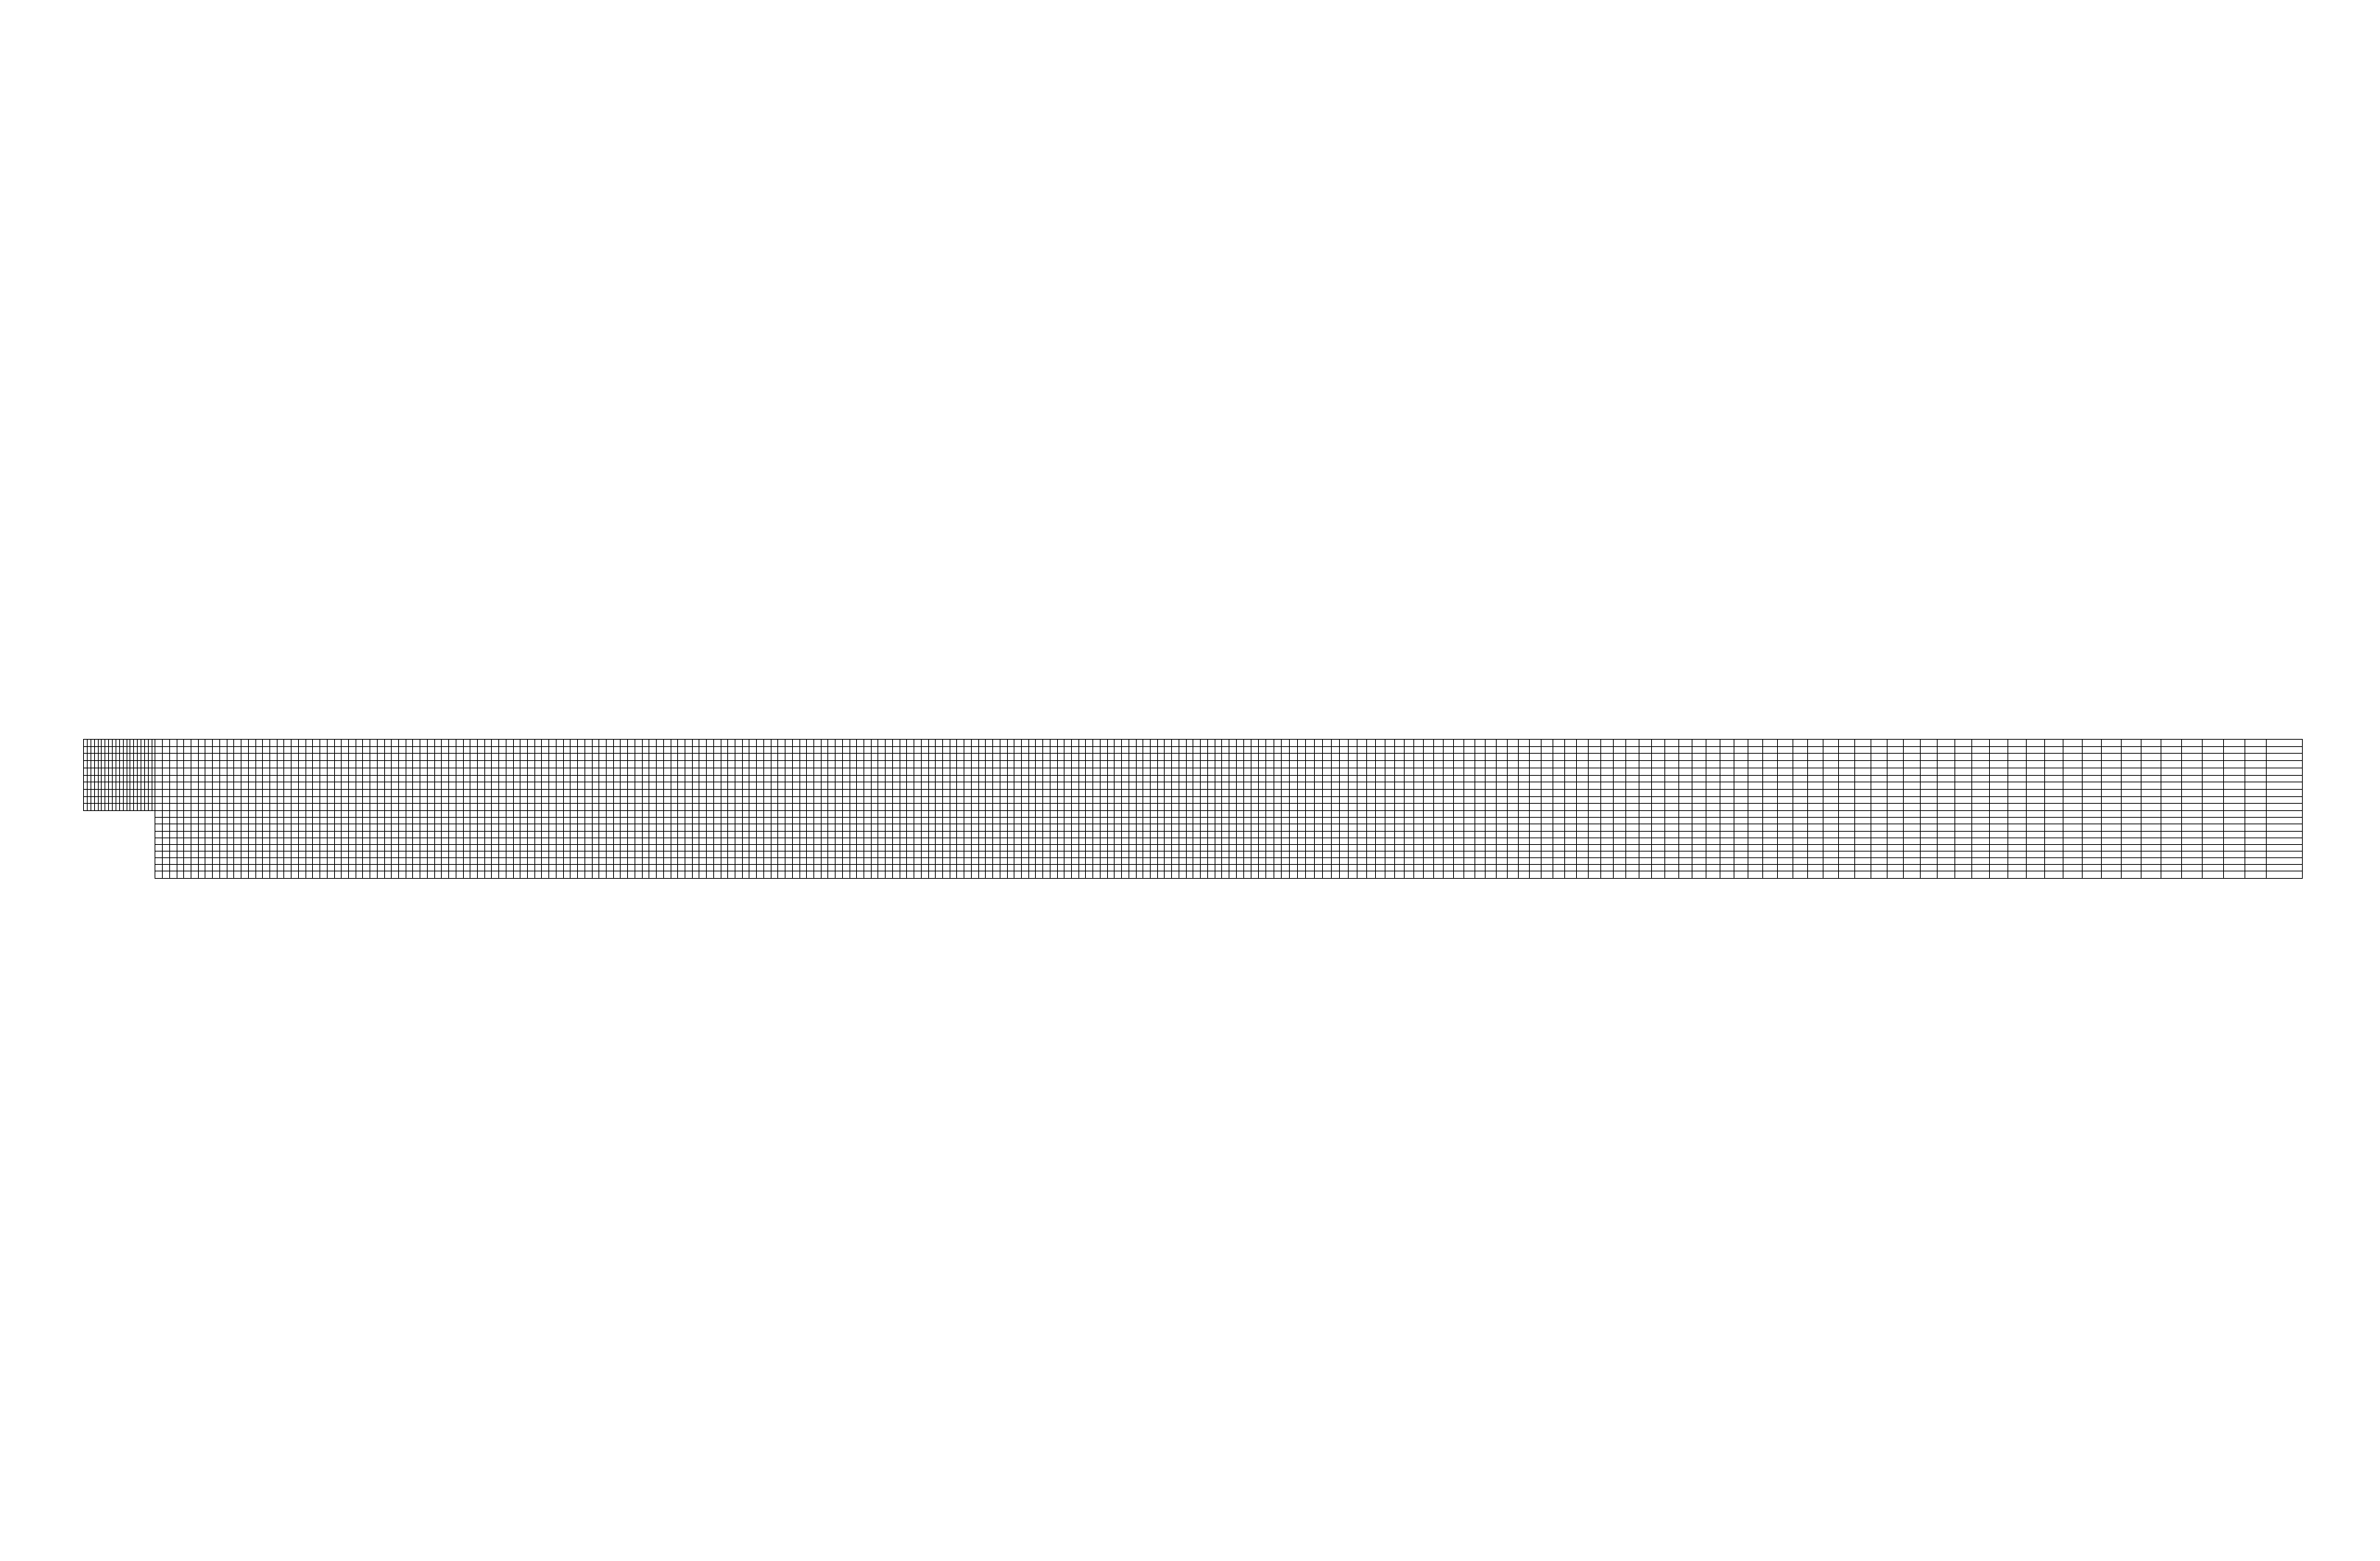
\includegraphics[scale=0.3,trim=1cm 14cm 1cm 14cm, clip=true]{Imagens/Cap2/malhadegrau.eps}
	\caption{Degrau 3D: Geometria e malha de células físicas}
	\label{fig:degrau_malha}
\end{figure}

\begin{center}
	\begin{table}[h!]
		\caption{Número de pontos de controle por \textit{patch}}
		\centering
		\begin{tabular}{|c | c | c| c|} 
			\hline
			\textit{Patch} & $\xi$ & $\eta$ & $\zeta$ \\ 
			\hline
			0 & 22 & 12 & 3 \\ 
			\hline
			1 & 152 & 12 & 3\\
			\hline
			2 & 152 & 12 & 3\\
			\hline
			3 & 82 & 12 & 3\\
			\hline
			4 & 82 & 12 & 3\\
			\hline
		\end{tabular}
		\label{tab:numberPCpatches}
	\end{table}
\end{center}


Na Fig. \ref{fig:degrau_com_recl} são apresentados os comprimentos de recolamento do vórtice primário adimensionalizados ($x_{r}/s$), juntamente com os resultados adaptados dos ensaios experimentais de \citeonline{ArmalyDP:1983} e os resultados de análises 2d de \citeonline{WilliamsB:1999}. Nota-se que os resultados obtidos estão próximos das referências para $\Reynolds = 100$ e $\Reynolds =400$, entretanto, para $\Reynolds = 800$ nota-se um afastamento do presente trabalho, e do referente à análise 2D com relação ao experimento realizado por \citeonline{ArmalyDP:1983}. Isto ocorre, visto que o ensaio experimental foi realizado com um canal com $2m$ de comprimento na direção $z$, e a simulação atual com apenas uma célula nessa direção é incapaz de captar os fenômenos tridimensionais que ocorrem a medida que o número de Reynolds cresce. Na Fig.\ref {fig:degrau_vortices} pode-se observar o campo de velocidade para os Reynolds estudados, e o aspecto do vórtice primário desenvolvido.


\begin{figure}[htb!]
	\centering
	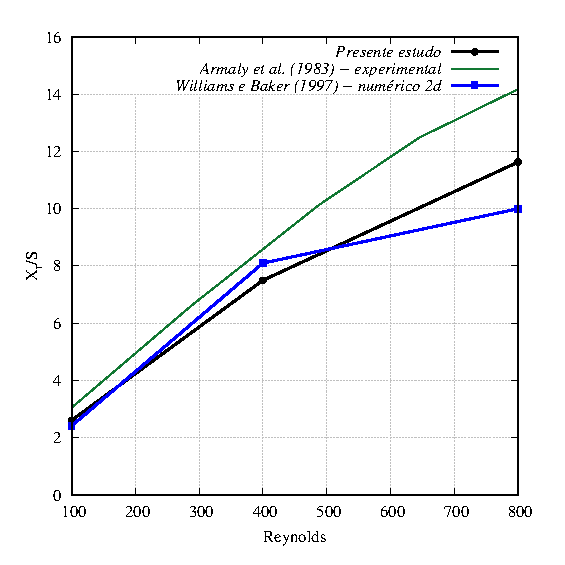
\includegraphics[scale=1.2,trim=0cm 0cm 0cm 0cm, clip=true]{Imagens/Cap2/comvort.eps}
	\caption{Degrau 3D: Comprimento de recolamento do v\'ortice principal}
	\label{fig:degrau_com_recl}
\end{figure}


\begin{figure}[!htb]
	\centering
	\subfloat[\label{fig:vortice_re100} $\Reynolds= 100$]{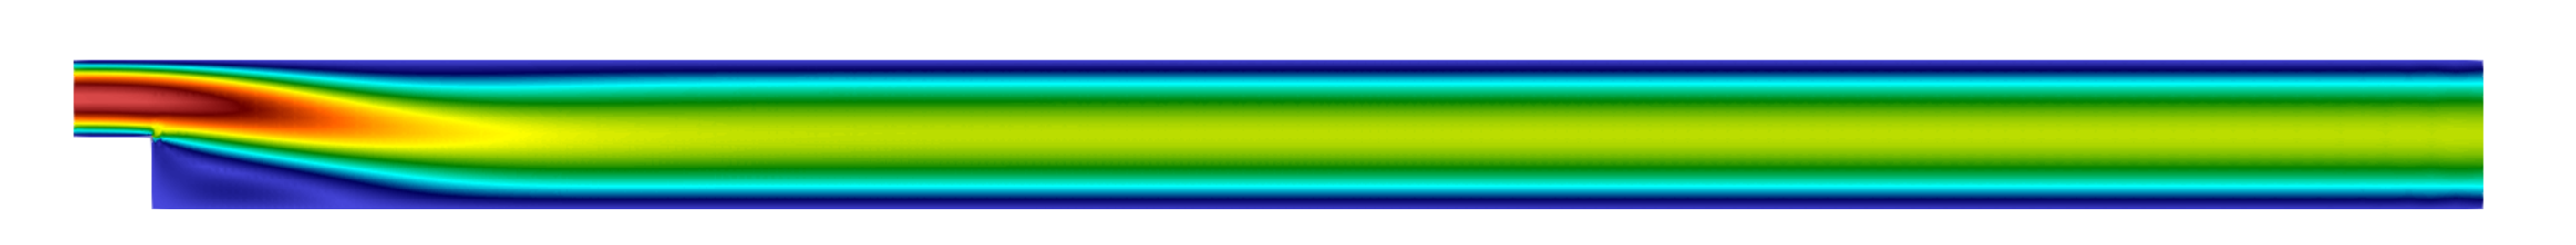
\includegraphics[scale=0.3,trim=0cm 0cm 0cm 0cm, clip=true]{Imagens/Cap2/degrau100.pdf}} \\
	\subfloat[\label{fig:vortice_re400} $\Reynolds= 400$]{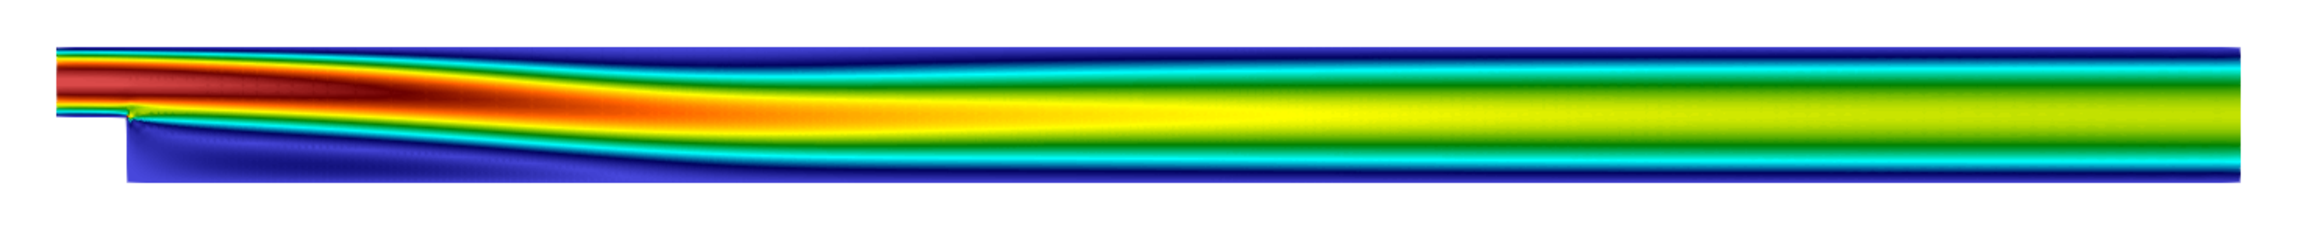
\includegraphics[scale=0.36,trim=0cm 0cm 0cm 0cm, clip=true]{Imagens/Cap2/degrau400.pdf}}\\ 
	\subfloat[\label{fig:vortice_re800}$\Reynolds= 800$]{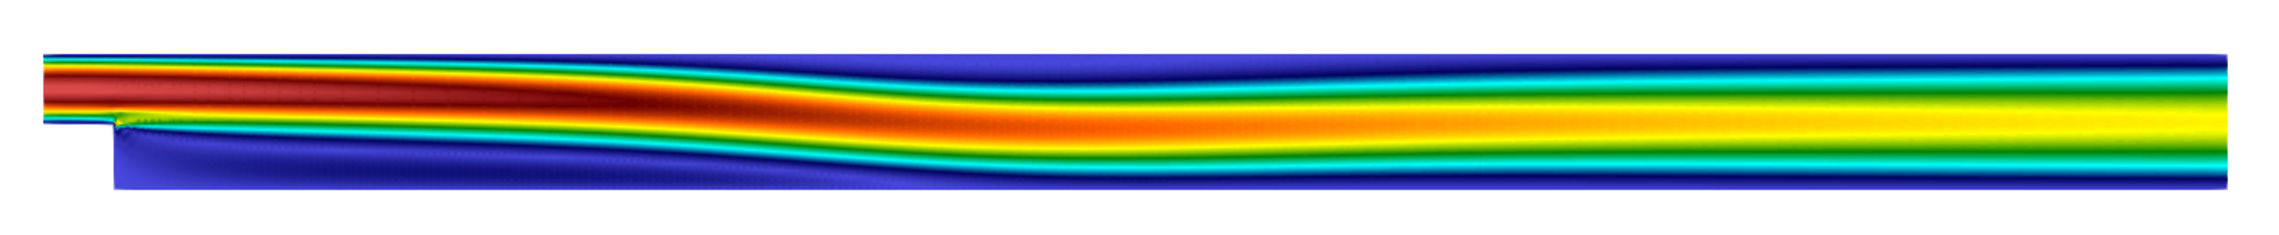
\includegraphics[scale=0.36,trim=0cm 0cm 0cm 0cm, clip=true]{Imagens/Cap2/degrau800.pdf}}\\
	{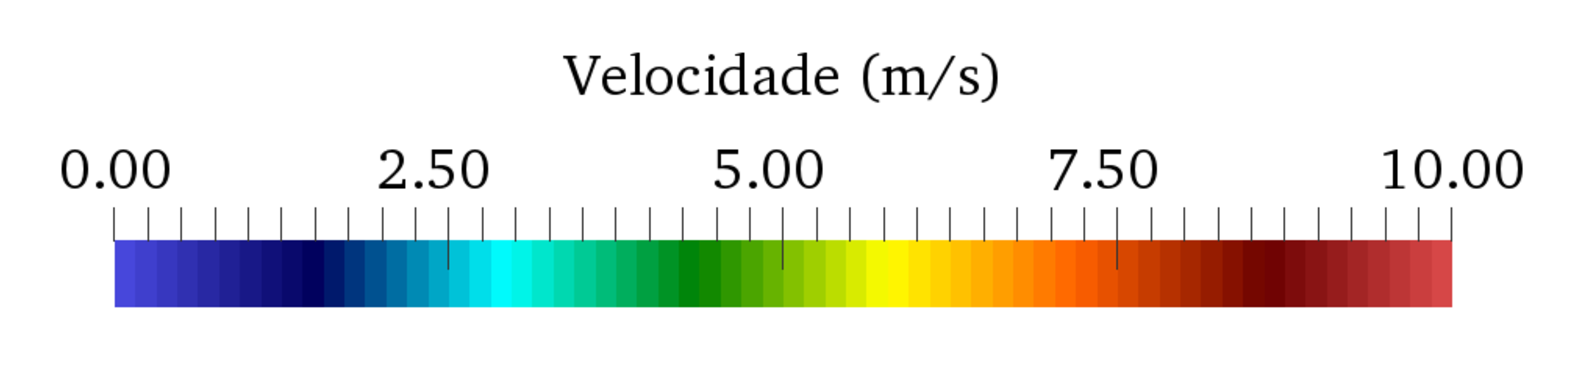
\includegraphics[scale=0.3,trim=0cm 0cm 0cm 0cm, clip=true]{Imagens/Cap2/legendadegrau.pdf}}
	\caption{Degrau 3D: Campo de velocidade. }
	\label{fig:degrau_vortices}
\end{figure}

\end{document}
